\section{Ridge, Lasso, and Elastic Net Regression}%
\label{sec:theory}

Throughout the paper we assume that the response \(\vec{y}\) is generated according to
\(y_i = \beta_0^* + \vec x_i^\T \vec\beta^* + \varepsilon_i\) for \(i \in [n]\) where \([n]
= \{1,2,\dots,n\}\), with \(\mat X\) being the \(n \times p\) design matrix with features
\(\vec x_j\) and where we assume \(\mat{X}\), \(\beta_0^*\), and \(\vec{\beta}^*\) to be
fixed. We will also assume that the features of the normalized design matrix are
orthogonal, that is, \(\tilde{\mat{X}}^\intercal \tilde{\mat{X}} =
\diag\left(\tilde{\vec{x}}_1^\T \tilde{\vec{x}}_1, \dots, \tilde{\vec{x}}_p^\intercal
\tilde{\vec{x}}_p\right)\). In this case, the solution to the coefficients in the elastic
net problem is given by
%
\begin{equation}
  \label{eq:orthogonal-solution-normalized}
  \hat{\beta}^{(n)}_j = \frac{\st_{\lambda_1}\left(\tilde{\vec{x}}_j^\T \vec{y}\right)}{\tilde{\vec{x}}_j^\T \tilde{\vec{x}}_j + \lambda_2},
  \qquad
  \hat{\beta}_0^{(n)} = \frac{\vec{y}^\T \ones}{n},
\end{equation}
%
where \(\st_\lambda(z)\) is the soft-thresholding operator, defined as \(\st_\lambda(z) =
\sign(z) \max(|z| - \lambda, 0)\). (See \Cref{sec:elastic-net-estimator} for a derivation
of this.)

Normalization changes the optimization problem and its solution, the coefficients, which
will now be on the scale of the normalized features. But we are interested in
\(\hat{\vec{\beta}}\): the coefficients on the scale of the original problem. To obtain
these, we transform the coefficients from the normalized problem, \(\hat\beta^{(n)}_j\),
back via \(\hat\beta_j = \hat\beta^{(n)}_j/s_j\) for \(j \in [p]\). There is a similar
transformation for the intercept but we omit here since we are not interested in
interpreting it.

Now assume that \(\varepsilon_i\) is identically and independently distributed noise with
mean zero and finite variance \(\sigma_\varepsilon^2\). This means that the solution is
given directly by \Cref{eq:orthogonal-solution-normalized}:
\[
  \hat{\beta}_j = \frac{\st_{\lambda_1}(\tilde{\vec{x}}_j^\T \vec{y})}{d_j}\quad\text{with}\quad d_j = s_j(\tilde{\vec{x}}_j^\T \tilde{\vec{x}}_j + \lambda_2).
\]
We can then show that
\begin{equation}
  \label{eq:z-d}
  \tilde{\vec{x}}_j^\T \vec{y} = \frac{\beta_j^* n \nu_j- \vec{x}_j^\T \vec{\varepsilon}}{s_j}
  \quad\text{and}\quad
  d_j = s_j\left(\frac{n \nu_j}{s_j^2} + \lambda_2\right),
\end{equation}
where \(\nu_j\) is the uncorrected sample variance of \(\vec{x}_j\).
The bias and variance of \(\hat{\beta}_j\) are then given by
\begin{align}
  % \bias(\hat{\beta}_j; \beta_j^*) & = \frac{1}{d_j}\E \st_\lambda(\tilde{\vec{x}}_j^\T \vec{y}) - \beta^*_j, \\
  \E \hat\beta_j - \beta_j^* & = \frac{1}{d_j}\E \st_\lambda(\tilde{\vec{x}}_j^\T \vec{y}) - \beta^*_j,\label{eq:bias} \\
  \var \hat\beta_j           & = \frac{1}{d_j^2} \var \st_\lambda(\tilde{\vec{x}}_j^\T \vec{y}).\label{eq:variance}
\end{align}
See \Cref{sec:bias-var-deriv} for a derivation of the results above
as well as expressions for \(\E \st_\lambda(x)\) and \(\var S_\lambda(x)\).

These expressions hold for a general distribution on the error term, provided that its
elements are independent and identically distributed. From now on, however, we will add the
assumption that \(\vec{\varepsilon}\) is normally distributed, under which both the bias
and variance of \(\hat{\beta}_j\) have analytical
expressions~(\Cref{sec:normally-distributed-noise}) and
\[
  \tilde{\vec{x}}_j^\T \vec{y} \sim \normal\left(\mu_j = \tilde{\vec{x}}_j^\T\vec{x}_j \beta_j^*, \sigma_j^2 = \tilde{\vec{x}}_j^\T\tilde{\vec{x}}_j \sigma_\varepsilon^2 \right).
\]

\subsection{Binary Features}%
\label{sec:theory-binary-features}

When \(x_{ij} \in \{0, 1\}\) for all \(i\), we define \(\bm{x}_j\) to be a \emph{binary
  feature}, and we define the \emph{class balance} of this feature as \(q_j =
\bar{\bm{x}}_j\): the proportion of ones. For most of our results, it would make no
difference if we were to swap the ones and zeros as long as an intercept is included, and
``class balance'' is then equivalent to the proportion of either. But in the case of
interactions~(\Cref{sec:interactions}), the choice matters.

If feature $j$ is binary then \(\nu_j = (q_j - q_j^2)\) (the uncorrected sample variance
for a binary feature) which in \Cref{eq:z-d} yields
\begin{align*}
  \tilde{\vec{x}}_j^\T \vec{y} & = \frac{\beta_j^* n(q_j - q_j^2) - \vec{x}_j^\T \vec{\varepsilon}}{s_j}, \\
  d_j                          & = s_j \left(\frac{n(q_j - q_j^2)}{s_j^2} + \lambda_2\right),
\end{align*}
% \[
%   \begin{aligned}
%     \tilde{\vec{x}}_j^\T \tilde{\vec{x}}_j & = \frac{1}{s_j^2}(\vec{x}_j - \ones c_j)^\T (\vec{x}_j - \ones c_j) = \frac{1}{s^2_j}(nq - 2nq_j^2 + nq_j^2) = \frac{nq_j(1-q_j)}{s^2_j}, \\
%     \tilde{\vec{x}}_j^\T \vec{x}_j         & = \frac{1}{s_j}(\vec{x}_j^\T \vec{x}_j - \vec{x}_j^\T \ones c_j) = \frac{nq_j(1 - q_j)}{s_j}.
%   \end{aligned}
% \]
and consequently
\[
  \mu_j = \frac{\beta^*_j n(q_j - q_j^2)}{s_j}\quad \text{and} \quad \sigma_j^2 = \frac{\sigma_\varepsilon^2n(q_j- q_j^2)}{s^2_j}.
\]
%
We obtain bias and variance of the estimator with respect to \(q_j\) by inserting
\(\tilde{\vec{x}}_j^\T \vec{y}\) and \(d_j\) into \Cref{eq:bias,eq:variance}.

The presence of the factor \(q_j - q_j^2\) in \(\mu_j\), \(\sigma_j^2\), and \(d_j\)
indicates a link between class balance and the elastic net estimator and that this
relationship is mediated by the scaling factor \(s_j\). To achieve some initial intuition
for this relationship, consider the noiseless case (\(\sigma_\varepsilon = 0\)) in which we
have
\begin{equation}
  \label{eq:noiseless-estimator}
  \hat{\beta}_j = \frac{\st_{\lambda_1}(\tilde{\vec{x}}_j^\intercal \vec{y})}{s_j\left(\tilde{\vec{x}}_j^\intercal \tilde{\vec{x}}_j + \lambda_2\right)}
  =
  \frac{\st_{\lambda_1}\left(\frac{\beta_j^* n (q_j - q_j^2)}{s_j}\right)}{s_j\left(\frac{n(q_j - q_j^2)}{s_j^2} + \lambda_2\right)}.
\end{equation}
%
This expression shows that class balance directly affects the estimator. For values of
\(q_j\) close to \(0\) or \(1\), the input into the soft-thresholding part of the estimator
diminishes and consequently forces the estimate to zero, that is, unless we use the scaling
factor \(s_j = q_j - q_j^2\), in which case the soft-thresholding part will be unaffected
by class imbalance. This choice will not, however, mitigate the impact of class imbalance
on the ridge part of the estimator, for which we would instead need \(s_j = (q_j -
q_j^2)^{1/2}\). For any other choices, \(q_j\) will affect the estimator through both the
ridge and lasso parts, which means that there exists no scaling \(s_j\) that will mitigate
this class balance bias in this case. In \Cref{sec:binary-weighting} we will show how to
tackle this issue for the elastic net by scaling the penalty weights. But for now we
continue to study the case of normalization.

Based on the reasoning above, we will consider the scaling parameterization \(s_j =
(q_j-q_j^2)^\delta\), \(\delta \geq 0\), which includes the cases that we are primarily
interested in, namely \(\delta = 0\) (no scaling, as in min--max and max--abs
normalization), \(\delta = 1/2\) (standard-deviation scaling), and \(\delta = 1\) (variance
scaling). The last of these, variance scaling, is not a standard type of normalization.

Another consequence of \Cref{eq:noiseless-estimator}, which holds also in the noisy
situation, is that normalization affects the estimator even when the binary feature is
balanced (\(q_j = 1/2\)). Using \(\delta = 0\), for instance, scales \(\beta_j^*\) in the
input to \(\st_\lambda\) by \(n (q_j - q_j^2) = n/4\). \(\delta = 1\), in contrast, imposes
no such scaling in the class-balanced case. And for \(\delta = 1/2\), the scaling factor is
\(n/2\). Generalizing this, we see that to achieve equivalent scaling in the class-balanced
case for all types of normalization, under our parameterization, we would need to use \(s_j
= 4^{\delta - 1} (q_j - q_j^2)^\delta\). But this only resolves the issue for the lasso. To
achieve a similar effect for ridge regression, we would need another (but similar)
modification. When all features are binary, we can just scale \(\lambda_1\) and
\(\lambda_2\) to account for this effect,\footnote{We use this strategy in all of the
  following examples.} which is equivalent to modifying \(s_j\). But when we consider mixes
of binary and normal features in \Cref{sec:mixed-data}, we need to exert extra care.

We now proceed to consider how class balance affects the bias, variance, and selection
probability of the elastic net estimator under the presence of noise. A consequence of our
assumption of a normal error distribution and consequent normal distribution of
\(\tilde{\vec{x}}_j^\T \vec{y}\) is that the probability of selection in the elastic net
problem is given by
\begin{align}
  \label{eq:selection-probability}
   & \Pr\left(\hat{\beta}_j \neq 0\right) =                                                                                                       \nonumber
  \\
  % & = \Pr\left(\st_{\lambda_1}({Z_j}) \neq 0\right)                                                                                                                                                                                                                           \nonumber \\
  %                                      & = \Pr\left({Z_j} > \lambda_1\right) + \Pr\left({Z_j} < -\lambda_1\right)                                                                                                                                                                                                  \nonumber \\
  %                                      & = \cdf\left(\frac{\mu_j - \lambda_1}{\sigma_j}\right) + \cdf\left(\frac{- \mu_j -\lambda_1}{\sigma_j}\right)                                                                                                                                                              \nonumber \\
   & \cdf \left( \frac{\beta_j^*n (q_j-q_j^2)^{1/2} - \lambda_1(q_j-q_j^2)^{\delta - 1/2}}{\sigma_\varepsilon \sqrt{n}}\right)                \nonumber     \\
   & + \cdf \left( \frac{-\beta_j^*n (q_j-q_j^2)^{1/2} - \lambda_1(q_j-q_j^2)^{\delta - 1/2}}{\sigma_\varepsilon \sqrt{n}}\right).
\end{align}
Letting \(\theta_j = -\mu_j - \lambda_1 \) and \(\gamma_j = \mu_j - \lambda_1\), we can
express this probability asymptotically as \(q_j \rightarrow 1^+\) as
\begin{equation}
  \label{eq:selection-probability-limit}
  \lim_{q_j \rightarrow 1^+} \Pr(\hat{\beta}_j \neq 0) =
  \begin{cases}
    0                                                                & \text{if } 0 \leq \delta < \frac{1}{2}, \\
    2\cdf\left(-\frac{\lambda_1}{\sigma_\varepsilon \sqrt{n}}\right) & \text{if } \delta = \frac{1}{2},        \\
    1                                                                & \text{if } \delta > \frac{1}{2}.
  \end{cases}
\end{equation}

In \Cref{fig:selection-probability}, we plot this probability for various settings of
\(\delta\) for a single feature. Our intuition from the noiseless case holds: suitable
choices of \(\delta\) can mitigate the influence of class imbalance on selection
probability. The lower the value of \(\delta\), the larger the effect of class imbalance
becomes. Note that the probability of selection initially decreases also in the case when
\(\delta \geq 1\). This is a consequence of increased variance of \(\tilde{\vec{x}}_j^\T
\vec{y}\) due to the scaling factor that inflates the noise term. But as \(q_j\) approaches
1, the probability eventually rises towards 1 for \(\delta \in \{1, 1.5\}\). The reason for
this is that this rise in variance eventually quells the soft-thresholding effect
altogether. Note, also, that the selection probability is unaffected by \(\lambda_2\).

\begin{figure}[htpb]
  \centering
  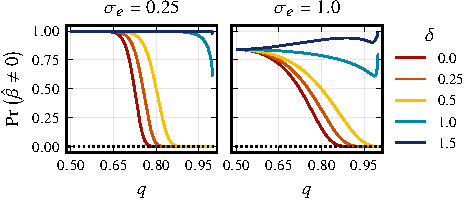
\includegraphics[]{plots/selection_probability.pdf}
  \caption{%
    Probability of selection in the lasso given measurement noise
    % TODO: what is \lambda1 set to here?
    \(\sigma_\varepsilon\), regularization level \(\lambda_1\), and class
    balance \(q\). The scaling factor is set to \(s_j = (q - q^2)^\delta\),
    \(\delta \geq 0\). The dotted line represents the asymptotic limit for
    \(\delta = 1/2\) from \Cref{eq:selection-probability-limit}.
    \label{fig:selection-probability}}
\end{figure}

% Now we turn to the impact of class imbalance on bias and variance of the elastic net
% estimator. We begin, in \Cref{thm:classbalance-bias}, by considering the expected value of
% the elastic net estimator in the limit as \(q_j \rightarrow 1^+\).

Now we turn to the impact of class balance on bias and variance of the elastic net
estimator.

\begin{theorem}
  \label{thm:classbalance-bias}
  If \(\vec{x}_j\) is a binary feature with class balance \(q_j \in (0, 1)\),
  \(\lambda_1 \in [0,\infty)\), \(\lambda_2 \in [0,\infty)\),
  \(\sigma_\varepsilon > 0\), and \(s_j = (q_j - q_j^2)^{\delta}\), \(\delta
  \geq 0\)  then
  \[
    \lim_{q_j \rightarrow 1^+} \E \hat{\beta}_j =
    \begin{cases}
      0                                                                                                  & \text{if } 0 \leq \delta < \frac{1}{2}, \\
      \frac{2n \beta_j^*}{n + \lambda_2} \cdf\left(-\frac{\lambda_1}{\sigma_\varepsilon \sqrt{n}}\right) & \text{if } \delta = \frac{1}{2},        \\
      \beta^*_j                                                                                          & \text{if } \delta > \frac{1}{2}.
    \end{cases}
  \]
\end{theorem}

\begin{theorem}
  \label{thm:classbalance-variance}
  Assume the conditions of \Cref{thm:classbalance-bias} hold, except that
  \(\lambda_1 > 0\). Then
  \[
    \lim_{q_j \rightarrow 1^+} \var \hat{\beta}_j =
    \begin{cases}
      0      & \text{if } 0 \leq \delta < \frac{1}{2}, \\
      \infty & \text{if } \delta \geq \frac{1}{2}.
    \end{cases}
  \]
\end{theorem}

The main take-away of \Cref{thm:classbalance-bias,thm:classbalance-variance} is that there
is a bias-variance trade-off with respect to the choice of normalization. We can reduce
class imbalance-induced bias by increasing \(\delta\) towards 1 (variance scaling) but do
so at the price of increase variance. Note that \Cref{thm:classbalance-variance} applies
only to the case when \(\lambda_1 > 1\). In
\Cref{cor:ridge-variance}~(\Cref{sec:ridge-variance}), we state the corresponding result
for ridge regression.

% shows that the
% bias of the elastic net estimator approaches \(-\beta_j^*\) as \(q_j \rightarrow 1^+\) when
% \(0 \leq \delta < 1/2\). When \(\delta = 1/2\) (standardization), the estimate instead
% approaches the true coefficient scaled by the probability that a standard normal variable
% is smaller than \(\beta_j^*\sqrt{n}\sigma_\varepsilon^{-1}\). For \(\delta > 1/2\), the
% estimate is asymptotically unbiased. This comes as a result of scaling the variance
% component from the error term and is accompanied by exponentially increasing variance,
% which suggests that variance-scaling may be problematic in the large noise--large imbalance
% scenario. In \Cref{thm:classbalance-variance}, we continue by studying the variance in the
% limit as \(q_j \rightarrow 1^+\).

% \Cref{thm:classbalance-bias,thm:classbalance-variance,cor:ridge-variance} shows that the bias of the elastic net estimator approaches
% \(-\beta_j^*\) as \(q_j \rightarrow 1^+\) when \(0 \leq \delta < 1/2\). When \(\delta =
% 1/2\) (standardization), the estimate instead approaches the true coefficient scaled by the
% probability that a standard normal variable is smaller than
% \(\beta_j^*\sqrt{n}\sigma_\varepsilon^{-1}\). For \(\delta > 1/2\), the estimate is
% asymptotically unbiased. This comes as a result of scaling the variance component from the
% error term and is accompanied by exponentially increasing variance, which suggests that
% variance-scaling may be problematic in the large noise--large imbalance scenario. In
% \Cref{thm:classbalance-variance}, we continue by studying the variance in the limit as
% \(q_j \rightarrow 1^+\).

% \Cref{thm:classbalance-variance} formally proves the asymptotic variance effects of our
% scaling parameter \(s_j\) which we have already discussed in the context of selection
% probability and bias. Taken together with the results from \Cref{thm:classbalance-bias},
% this suggests that the choice of scaling parameter, at least in the case of our specific
% parameterization, introduces a bias--variance trade-off with respect to \(\delta\): we can
% reduce class imbalance-induced bias by increasing \(\delta\) but do so at the price of
% increase variance.

In \Cref{fig:bias-var-onedim-lasso}, we now visualize bias, variance, and mean-squared
error for ranges of class balance and various noise-level settings for a lasso problem. The
figure demonstrates the bias--variance trade-off that our asymptotic results suggest and
indicates that the optimal choice of \(\delta\) is related to the noise level in the data.
Since this level is typically unknown and can only be reliably estimated in the
low-dimensional setting, it suggests there might be value in selecting \(\delta\) through
hyper-optimization. In
\Cref{fig:bias-var-onedim-ridge-full}~(\Cref{sec:additional-results-biasvar}) we show
results for ridge regression as well. As expected, it is then \(\delta = 1/2\) that leads
to unbiased estimates in this case. Also see
\Cref{fig:bias-var-onedim-lasso-full}~(\Cref{sec:additional-results-biasvar}) for extended
results on the lasso.

\begin{figure}[htb]
  \centering
  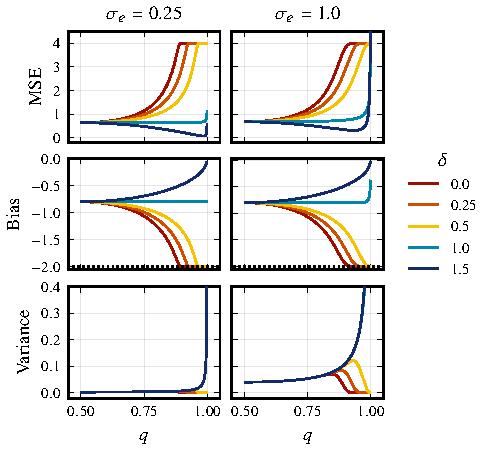
\includegraphics[]{plots/binary_onedim_bias_var_lasso_small.pdf}
  \caption{%
    Bias, variance, and mean-squared error for a one-dimensional lasso problem,
    parameterized by noise level (\(\sigma_\varepsilon\)), class balance (\(q\)), and
    scaling (\(\delta\)). Dotted lines represent asymptotic bias of the lasso
    estimator in the case when \(\delta = 1/2\).}
  \label{fig:bias-var-onedim-lasso}
\end{figure}

So far, we have only considered a single binary feature, but in
\Cref{sec:power-fdr-multiple} we present results on power and false discovery rates for a
problem with multiple features.

\subsection{Mixed Data}%
\label{sec:mixed-data}

A fundamental problem with mixes of binary and continuous features is deciding how to put
these features on the same scale in order to regularize each type of feature fairly. In
principle, we need to match a one-unit change in the binary feature with some amount of
change in the normal feature. This problem has previously been tackled, albeit from a
different angle, by \citet{gelman2008}, who argued that the common default choice of
presenting standardized regression coefficients unduly emphasizes coefficients from
continuous features.

To setup this situation formally, we will say that the effects of a binary feature
\(\vec{x}_1\) and a normal feature \(\vec{x}_2\) are \emph{comparable} if \(\beta^*_1 =
\kappa \sigma \beta^*_2\), where \(\kappa > 0\) represents the number of standard
deviations of the normal feature we consider to be comparable to one unit on the binary
feature. As an example, assume \(\kappa = 2\). Then, if \(\vec{x}_2\) is sampled from
\(\normal\left(\mu_j, \sigma^2 = (1/2)^2\right)\), the effects of \(\vec{x}_1\) and
\(\vec{x}_2\) are comparable if \(\beta_1^* = 2\sigma \beta_2^* = \beta_2^*\).

% We illustrate this notion of comparability by the following examples.
% TODO: illustrate this with a figure
% \begin{example}
%   Assume \(\kappa = 2\). If \(\vec{x}_2\) is sampled from
%   \(\normal\left(\mu_j, \sigma^2 = (1/2)^2\right)\), then the effects of \(\vec{x}_1\) and
%   \(\vec{x}_2\) are comparable if \(\beta_1^* = 2\sigma \beta_2^* = \beta_2^*\).
% \end{example}
% \begin{example}
%   Assume \(\kappa = 1\). If \(\vec{x}_2\) is sampled from \(\normal(\mu,
%   \sigma^2 = 2^2)\), then the effects of \(\vec{x}_1\) and \(\vec{x}_2\) are comparable if
%   \(\beta_1^* = \sigma\beta_2^* = 2\beta_2^*\).
% \end{example}

The definition above refers to \(\bm{\beta}^*\), but for our regularized estimates we need
\(\hat{\beta}_1 = \kappa\sigma\hat{\beta}_2\) to hold. If we assume that we are in a
noiseless situation (\(\sigma_\varepsilon = 0\)), are standardizing the normal feature, and
that, without loss of generality, \(\bar{x}_1 = 0\), then we need the following equality to
hold:
%
\begin{align}
  \label{eq:comparable-effects}
  \hat{\beta}_1                                                                                                                          & = \kappa\sigma \hat{\beta}_2                                                                                                                         & \implies \nonumber \\
  \frac{\st_{\lambda_1}(\tilde{\vec{x}}_1^\intercal \vec{y})}{s_1\left(\tilde{\vec{x}}_1^\intercal \tilde{\vec{x}}_1 + \lambda_2\right)} & =\frac{\kappa\sigma \st_{\lambda_1}(\tilde{\vec{x}}_2^\intercal \vec{y})}{s_2\left(\tilde{\vec{x}}_2^\intercal \tilde{\vec{x}}_2 + \lambda_2\right)} & \implies \nonumber \\
  \frac{\st_{\lambda_1}\left(\frac{n\beta_1^* (q - q^2)}{s_1}\right)}{s_1\left(\frac{n(q - q^2)}{s_1^2} + \lambda_2\right)}              & =  \frac{\kappa \st_{\lambda_1}\left(\frac{n\beta_1^*}{\kappa} \right)}{n + \lambda_2}.                                                              &
\end{align}

For the lasso (\(\lambda_2 = 0\)) and ridge regression (\(\lambda_1=0\)), we see that the
equation holds for \(s_1 = \kappa (q - q^2)\) and \(s_1 = (q - q^2)^{1/2}\), respectively.
In other words, we achieve comparability in the lasso by scaling each binary feature with
its variance times \(\kappa\). And for ridge regression, we can achieve comparability by
scaling with standard deviation, irrespective of \(\kappa\). For any other choices of
\(s_1\), equality holds only at a fixed level of class balance. Let this level be \(q_0\).
Then, to achieve equality for \(\lambda_2 = 0\), we need \(s_1 =\kappa (q_0 - q_0^2)^{1 -
  \delta}(q - q^2)^\delta\). Similarly, for \(\lambda_1 = 0\), we need \(s_1 = (q_0 -
q_0^2)^{1 - 2\delta} (q - q^2)^\delta\). In the sequel, we will assume that \(q_0 = 1/2\),
to have effects be equivalent for the class-balanced case.

Note that this means that the choice of normalization has an implicit effect on the
relative penalization of binary and normal features, even in the class-balanced case (\(q_1
= 1/2\)). If we for instance use \(\delta=0\) and fit the lasso, then
\Cref{eq:comparable-effects} for a binary feature with \(q_1=1/2\) becomes
\(4\st_{\lambda_1}\left(n\beta_1^*/4\right) = \kappa \st_{\lambda_1}(n\beta_1^*/\kappa ),\)
which implies \(\kappa = 4\). In other words, the choice of normalization equips our model
with a belief about how binary and normal features should be penalized relative to one
another.

For the rest of this paper, we will use \(\kappa = 2\) and say that the effects are
comparable if the effect of a flip in the binary feature equals the effect of a
two-standard deviation change in the normal feature. We motivate this by an argument by
\citet{gelman2008}, but want to stress that the choice of \(\kappa\) should, if possible,
be based on contextual knowledge of the data and that our results depend only superficially
on this particular setting.
% We do, however, want to emphasize that this choice should be made
% \emph{actively} and not be allowed to implicitly depend on the type of normalization used.

% Finally, note that we assumed a noiseless case above. In the presence of noise, the bias
% induced by the combination of noise level and normalization choice will affect these
% results (see \Cref{fig:bias-var-onedim-lasso}), which means that normally distributed and
% binary features will not be comparable in this case.

\subsection{Interactions}\label{sec:interactions}

The elastic net can be extended to include interactions. There is previous literature on
this topic~\citep{bien2013,zemlianskaia2022,lim2015}, but it has not considered the
possible influence of normalization. Here, we will consider simple pairwise interactions
with no restriction on the presence of main effects. For our analysis, we let \(\vec{x}_1\)
and \(\vec{x}_2\) be two features of the data and \(\bm{x}_3\) their interaction, so that
\(\beta_3\) represents the interaction effect.

We consider two cases in which we assume that the features are orthogonal and that
\(\vec{x}_1\) is binary with class balance \(q_1\). In the first case, we let \(\bm{x}_2\)
be normal with mean \(\mu\) and variance \(\sigma^2\), and in the second case \(\bm{x}_2\)
be binary with class balance \(q_2\). To construct the interaction feature, we
center\footnote{See \Cref{sec:centering-interactions} for motivation for why we center the
  features before computing the interaction.} the main features and then multiply
element-wise. The elements of the interaction feature are then given by \(x_{3,i} =
(x_{1,i} - \bar{\bm{x}}_1)(x_{2,i} - \bar{\bm{x}}_2)\).

If \(\bm{x}_2\) is normal and both features are centered before computing the interaction
term, the variance becomes \(\sigma^2 (q-q^2)\), which suggests using \(s_3 = \sigma (q -
q^2)^\delta\) along the lines of our previous reasoning. And if \(\bm{x}_2\) is binary,
instead, then similar reasoning suggests using \(s_3 = ((q_1-q_1^2)(q_2-q_2^2))^\delta\).
In \Cref{sec:experiments-interactions}, we study the effects of these choices in simulated
experiments.

\subsection{The Weighted Elastic Net}\label{sec:binary-weighting}

We have so far shown that certain choices of normalization can mitigate the class-balance
bias imposed by the lasso and ridge regularization. But we have also
demonstrated~(\Cref{sec:theory-binary-features}) that there is no (simple) choice of
scaling that can achieve the same effect for the elastic net.
\Cref{eq:noiseless-estimator}, however, suggests a natural alternative to normalization,
which is to use the weighted elastic net, in which we minimize
\[
  \frac{1}{2} \lVert \vec{y} - \beta_0 - \mat{X}\vec{\beta}\rVert_2^2 + \lambda_1 \sum_{j=1}^p u_j |\beta_j| + \frac{\lambda_2}{2} \sum_{j=1}^p v_j \beta_j^2,
\]
with \(\vec{u}\) and \(\vec{v}\) being \(p\)-length vectors of positive scaling factors.
This is equivalent to the standard elastic net for a normalized feature matrix when \(u_j =
s_j\) and \(v_j = s_j^2\), which can be seen by substituting \(\beta_js_j =
\tilde{\beta}_j\) in \Cref{eq:elastic-net} and solving for \(\tilde{\vec{\beta}}\). Note
that we do not need to rescale the coefficients from this problem as we would for the
standard elastic net on normalized data.

This allows us to control class-balance bias by setting our weights according to \(u_j =
v_j = (q_j - q_j^2)^{\omega}\) and counteract it, at least in the noiseless case, with
\(\omega = 1\), which, we want to emphasize, is \emph{not} possible using the standard
elastic net. For the lasso and ridge regression, however, this setting of \(\omega=1\) is
equivalent to using \(\delta = 1\) and \(\delta = 1/2\), respectively, in the standard
elastic net with normalized data.

Results analogous to those in \Cref{sec:theory-binary-features} can be attained with a few
small modifications for the weighted elastic net case. Starting with selection probability,
we can set \(s_j = 1\) and replace \(\lambda_1\) with \(\lambda_1 u_j =
\lambda_1(q_j-q_j^2)^\omega\) in \Cref{eq:selection-probability}, which shows that
\(\omega\) and \(\delta\) have interchangeable effects for selection probability.

As far as expected value and variance of the weighted elastic net estimator is concerned,
the same expressions apply directly in the case of the weighted elastic net given \(s_j =
1\) for all \(j\) and replacing \(\lambda_1\) as in the previous paragraph and
\(\lambda_2\) with \(\lambda_2 (q_j - q_j^2)^\omega\). On the other hand, the asymptotic
results differ slightly as we now show.

\begin{theorem}
  \label{thm:weighted-elasticnet-bias-variance}
  Let \(\vec{x}_j\) be a binary feature with class balance \(q_j \in (0, 1)\) and take
  \(\lambda_1 > 0\), \(\lambda_2 > 0\), and \(\sigma_\varepsilon > 0\). For the
  weighted elastic net with weights \(u_j = v_j = (q_j-q_j^2)^\omega\) and \(\omega \geq 0\), it holds that
  \[
    \lim_{q_j \rightarrow 1^+} \E \hat{\beta}_j =
    \begin{cases}
      0                              & \text{if } 0 \leq \omega < 1, \\
      \frac{\beta^*n}{n + \lambda_2} & \text{if } \omega = 1,        \\
      \beta^*                        & \text{if } \omega > 1,
    \end{cases}
  \]
  \[
    \lim_{q_j \rightarrow 1^+} \var \hat{\beta}_j =
    \begin{cases}
      0      & \text{if } 0 \leq \delta < \frac{1}{2}, \\
      \infty & \text{if } \delta \geq \frac{1}{2}.
    \end{cases}
  \]
\end{theorem}

This result for expected value is similar to the one for the unweighted but normalized
elastic net. The only difference arises in the case when \(\omega = 1\), in which case the
limit is unaffected by \(\lambda_1\) in the case of the weighted elastic net. For variance,
the result mimics the result for the elastic net with normalization.

The results for bias, variance, and mean-squared error for the weighted elastic net are
similar to those in \Cref{fig:bias-var-onedim-lasso} and are plotted in
\Cref{fig:binary-onedim-bias-var-elnet}~(\Cref{sec:additional-results-biasvar}).
